\documentclass[../main]{subfiles}
\usepackage{lastpage,xr,refcount,etoolbox}
% \externaldocument{references}
\begin{document}


\chapter{What is Machine Learning}

{
\hypersetup{linkcolor=black}
\minitoc
}


Machine learning is a branch of artificial intelligence that enables systems to learn from and make decisions based on data without explicit programming. Instead of following fixed instructions, machine learning algorithms analyze data to identify patterns and improve their performance over time.

This field encompasses various techniques such as supervised learning, where models are trained on labeled data, and unsupervised learning, where models uncover hidden patterns in unlabeled data. Reinforcement learning, another approach, involves models learning through interaction and feedback.

Applications of machine learning are widespread, including healthcare for predicting diseases and personalizing treatments; finance for detecting fraud and optimizing trading; and everyday technology, such as recommendation systems on streaming platforms. To effectively grasp machine learning, it's important to start with the basics, such as understanding the perceptron, which serves as a foundational concept for more advanced models.

\section{The perceptron}

A perceptron is a fundamental building block in machine learning and neural networks, often used as a basic unit for binary classification tasks. It is the simplest type of artificial neural network. A perceptron is a linear classifier that classifies data into one of two categories. It operates by taking a set of input features, applying weights to these features, and then passing the weighted sum through an activation function to produce an output.
\begin{figure}[H]
  \centering
  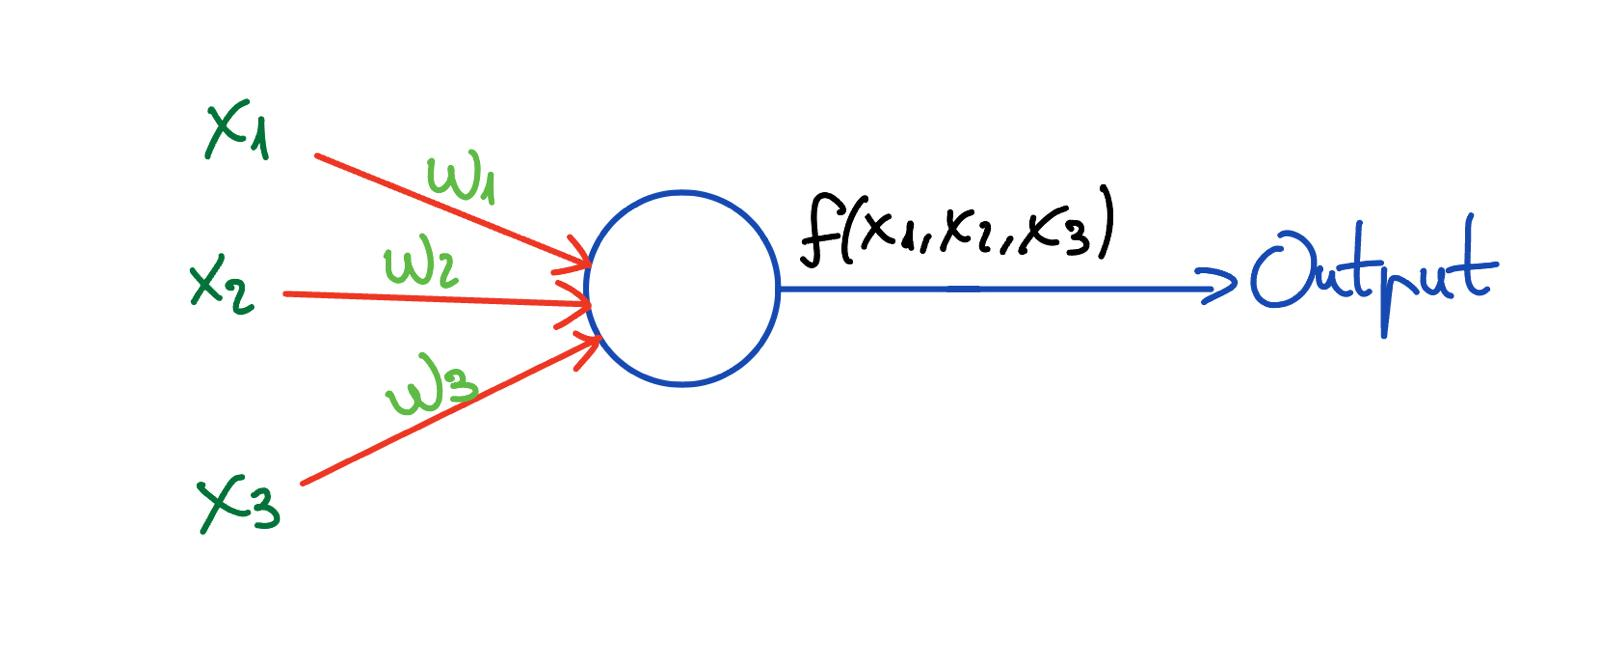
\includegraphics[width=0.4\textwidth]{./figures/perceptron}
  \caption{The perceptron}
  \label{fig:red}
\end{figure}
\begin{equation*}
    Output = f(x_1, x_2, x_3) = \begin{cases}
  \ 0 \ \ & \text{if } \ \ (\Sigma_iw_ix_i) + threshold \leq 0 \\
  \ 1 \ & \text{if } \ \ (\Sigma_iw_ix_i) + threshold > 0
\end{cases}
\end{equation*}

We can simplify the mathematical description of perceptrons. Let $\Sigma_iw_i x_i$ be defined as the vector dot product of the input vector and the vector of weights of the perceptron. Additionally, we will replace the threshold notation with b. This b represents how easily the perceptron outputs a 1 (bias).
\begin{equation*}
    Output = \begin{cases}
  \ 0 \ \ & \text{if } \ \ w\cdot x + b \leq 0 \\
  \ 1 \ & \text{if } \ \ w\cdot x + b > 0
\end{cases}
\end{equation*}
\section{The sigmoid neuron}
A single perceptron is not particularly useful on its own. To perform complex tasks similar to those handled by the human brain, an intriguing approach is to connect multiple perceptrons together, using the outputs of some as inputs to others. However, regardless of how sophisticated the architecture is, perceptrons are limited by their binary outputs, making them vulnerable to small disturbances.

We can address this issue by introducing a new type of artificial neuron known as a sigmoid neuron. These networks are similar to perceptrons, but they use a smoothing activation function (the sigmoid function) to produce their outputs.
\begin{equation*}
    Output = \sigma (\Sigma_iw_ix_i+b)= \sigma(w\cdotx+b)
\end{equation*}
\begin{equation*}
    \sigma(z) = \frac{1}{1+e^{-z}} \ \ \ | \ \ \ \sigma(z) \in [0, 1] \ \ \forall z \in \mathcal{R}
\end{equation*}
\begin{figure}[H]
  \centering
  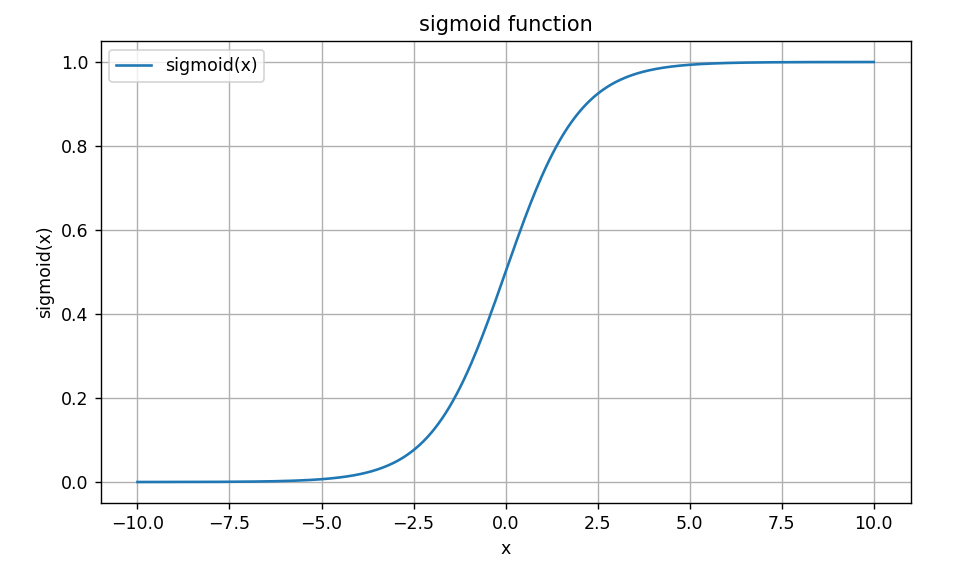
\includegraphics[width=1\textwidth]{./figures/sigmoid}
  \caption{The Sigmoid Function}
  \label{fig:red}
\end{figure}
There are many activation functions, each suited for different tasks. However, from now on, when I refer to the activation function, I will be talking about the sigmoid function. If we combine multiple sigmoid neurons, we have a mathematical device capable of performing more complex tasks, but how do these multilayer sigmoid perceptron networks calculate an output?
\section{Forward Propagation}
Now that we have established that the neural networks we will work with, are indeed multilayer sigmoid perceptron networks, we need to formally define their structure and how to evaluate them. The notation is as follows: we will use $w_{ik}^{l}$ to denote the weight for the connection between the $k^{th}$ neuron in the $(l-1)^{th}$ layer and the $i^{th}$ neuron in the $l^{th}$ layer. Similarly, we will use $b_{i}^{l}$ for the bias of the $i^{th}$ neuron in the $l^{th}$ layer and $x_{i}^{l}$ for the input of the $i^{th}$ neuron in the $l^{th}$ layer.
\begin{figure}[H]
  \centering
  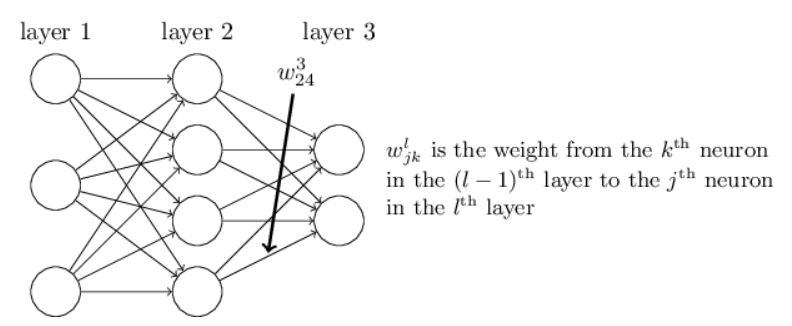
\includegraphics[width=1\textwidth]{./figures/network}
  \caption{Network notation (figure extracted from Michael Nielsen's book)}
  \label{fig:red}
\end{figure}
Having established the nomenclature, we now possess the necessary tools to formally express the output of a layer in the network. Specifically, in the context of a linear network, we can represent the output of the $l^{th}$ layer as a linear transformation of the input, utilizing the respective weights and biases:
\begin{equation*}
\begin{pmatrix}
x_{1}^i \vspace{0.15cm}\\ 
x_{2}^i \vspace{0.15cm}\\ 
...     \vspace{0.15cm}\\
x_{n}^i
\end{pmatrix} = \sigma \left(
\begin{pmatrix}
w_{1,1}^i & w_{2,1}^i & ... & w_{r,1}^i\vspace{0.15cm}\\ 
w_{1,2}^i & w_{2,2}^i & ... & w_{r,2}^i\vspace{0.15cm}\\ 
...       & ...       & ... & ...\vspace{0.15cm}\\
w_{1,n}^i & w_{2,n}^i & ... & w_{r,n}^i
\end{pmatrix}\cdot
\begin{pmatrix}
x_{1}^{i-1} \vspace{0.15cm}\\ 
x_{2}^{i-1} \vspace{0.15cm}\\ 
...     \vspace{0.15cm}\\
x_{r}^{i-1}
\end{pmatrix}+
\begin{pmatrix}
b_{1}^{i} \vspace{0.15cm}\\ 
b_{2}^{i} \vspace{0.15cm}\\ 
...     \vspace{0.15cm}\\
b_{n}^{i}
\end{pmatrix}\right)
\end{equation*}
We can also simplify the mathematical notation by using vector notation. In this way, the function that calculates the forward propagation would look like this (where $w^i \cdot x^{i-1}$ represents a matrix multiplication):
\begin{equation*}
    f(x^i) = \begin{cases}
  \ \sigma(w^i\cdot x^{i-1}+b^i) \ \ & \text{if } \ \ i > 1 \\
  \ x^i \ & \text{if } \ \ i = 1
\end{cases}
\end{equation*}
\section{Code of the Neural Network}
In this section, we showcase and explain the code for the constructor of our Neural Network object, as well as the implementation of the forward propagation function. First, we import the necessary libraries:
\begin{lstlisting}
import numpy as np
import random
\end{lstlisting}
The next step is to implement at least the sigmoid activation function, which will be used as the default:
\begin{lstlisting}
def sigmoid(z: float) -> float:
    return 1.0/(1.0+np.exp(-z))
\end{lstlisting}
Since Python is an object-oriented language, we will encapsulate all the information and routines of our neural network within a Python class:
\begin{lstlisting}
class Network(object):
\end{lstlisting}

The constructor of our Network takes a list specifying its shape (sizes) and constructs the weights and biases matrices. For example, if sizes = [2, 4, 6], it represents a neural network with three layers: the first layer having 2 neurons, the second layer having 4 neurons, and the third layer having 6 neurons:
\begin{lstlisting}
def __init__(self, sizes: List[int]):
    # Dimensions of the neural network
    self.num_layers = len(sizes)
    # Number of layers in the neural network
    self.sizes = sizes

    self.biases = [np.random.randn(y, 1) for y in sizes[1:]]
    self.weights = [np.random.randn(y, x) for x, y in zip(sizes[:-1], sizes[1:])]
    
    # np.random.rand(a, b) generates a matrix with a rows and b columns with random values
    # sizes[1:] is a list with all the elements in sizes except for the first one
    # sizes[:-1] is a list with all the elements in sizes except for the last one
\end{lstlisting}
Since the weights and biases matrices are well-defined, implementing the forward propagation function is straightforward, using the mathematical definitions provided earlier:
\begin{lstlisting}
def forward_propagation(self, input, activation=sigmoid):
        for b, w in zip(self.biases, self.weights):
            input = activation(w @ input + b)
            # @ is the matrix multiplication operator
        return input
\end{lstlisting}
\end{document}


%\hyperlink{target:zona}{\textcolor{blue}{[2]}} 